\documentclass[letterpaper,11pt]{article}
\usepackage[utf8]{inputenc} 
\usepackage{amsmath}
\usepackage{geometry}
\usepackage{graphicx}
\usepackage{tikz}
\usepackage{xcolor}
\usetikzlibrary{shapes.geometric, arrows, positioning}
\geometry{margin=2.5cm}



\tikzstyle{block} = [rectangle, rounded corners, minimum width=3cm, minimum height=1cm,text centered, draw=black, fill=blue!20]
\tikzstyle{input} = [block, fill=yellow!30]
\tikzstyle{output} = [block, fill=green!30]
\tikzstyle{arrow} = [thick,->,>=stealth]



\title{\textbf{Research Project Prototype\\Version 1}}
\author{} 
\date{\today}


\begin{document}

\maketitle
\hrulefill
\tableofcontents
\vfill

\section{Introduction}
One of the first and most important approaches to the Research Project is to build an initial prototype to confirm the feasibility of the project and identify potential flaws. In this report, the goal is to synthetically discuss the methodology, the results, and conclude about the first prototype to move forward with the overall project and ensure to start with strong foundations.
\begin{center}
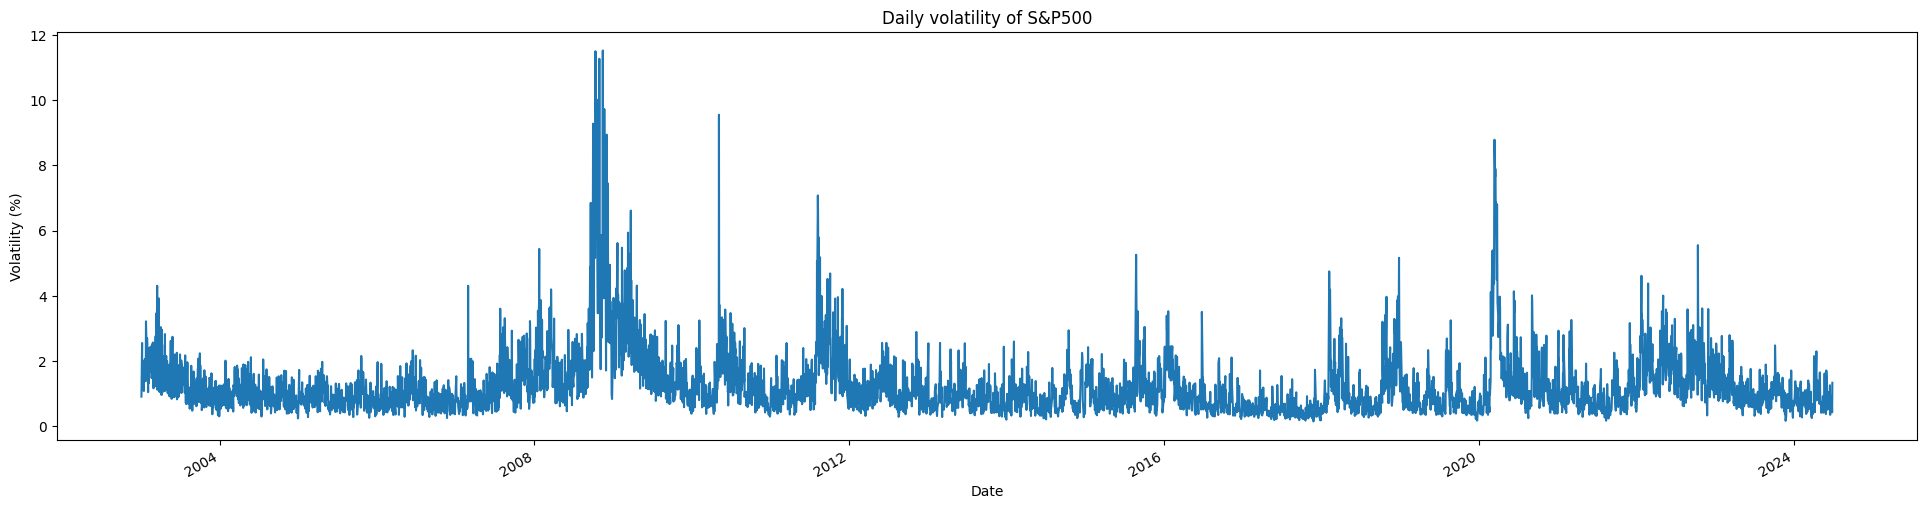
\includegraphics[width=0.9\textwidth]{img/vol500.png}
\end{center}
\newpage

\section{Methodology}

\subsection{Data}

Data is a key aspect of ANN results. To ensure data quality, I went through a data preprocessing script, "dataPreprocessing.ipynb." Alongside having clean data, it is crucial to have proper features to train the models. Their importance is defined by their correlation with the target. For volatility, the price of the last traded options or market data may be very relevant. All the classified features impacting volatility can be found in the document "volatility.html."  
The data is downloaded within the code using yfinance, and some, like economic indicators, are downloaded manually from the FRED website.\\
For this prototype and to gain simplicity and time, I have used Python for data treatment and analysis. I might use R in the future, depending on the pros and cons.  
Below is a data dictionary of the df after data gathering and preprocessing, before being split by the ANN:

\begin{table}[ht]
\centering
\caption{Data Dictionary}
\begin{tabular}{|l|l|l|p{7cm}|}
\hline
\textbf{Type} & \textbf{Column} & \textbf{Data Type} & \textbf{Description} \\ \hline
Feature & Date & datetime64[ns] & The date of the record. \\ \hline
Feature & Inflation & float64 & The inflation rate at the given date. \\ \hline
Feature & CPI & float64 & Consumer Price Index (CPI) value. \\ \hline
Feature & Treasury\_Yield & float64 & Yield on 10-year Treasury bonds. \\ \hline
Feature & Open & float64 & Opening value of the S\&P500 index. \\ \hline
Feature & High & float64 & Max S\&P500 price during the day. \\ \hline
Feature & Low & float64 & Min S\&P500 price during the day. \\ \hline
Feature & Close & float64 & Closing value of S\&P500. \\ \hline
Feature & SP500\_Adj\_Close & float64 & Adjusted closing value of S\&P500. \\ \hline
Feature & Volume & int64 & Volume of trades in the S\&P 500 index. \\ \hline
Feature & GDP & float64 & Gross Domestic Product value. \\ \hline
Feature & mortage & float64 & Average mortgage rate. \\ \hline
Feature & unemployement & float64 & Unemployment rate. \\ \hline
Feature & fed\_fund\_rate & float64 & Federal funds rate. \\ \hline
Feature & volatility & float64 & Historical volatility of the S\&P500 index. \\ \hline
\textbf{Target} & volatility\_forcast & float64 & Forecasted volatility of the S\&P 500. \\ \hline
Feature & returns & float64 & Logarithmic returns of the S\&P 500 index. \\ \hline
Feature & EWMA\_VM & float64 & Exponentially weighted moving average. \\ \hline
Feature & GARCH\_VM & float64 & GARCH volatility measure. \\ \hline
Feature & EGARCH\_VM & float64 & EGARCH volatility measure. \\ \hline
Feature & RogersSatchell\_VM & float64 & Rogers-Satchell volatility measure. \\ \hline
Feature & garman\_klass & float64 & Garman-Klass volatility measure. \\ \hline
Feature & parkinson & float64 & Parkinson volatility measure. \\ \hline
Feature & yang\_zhang & float64 & Yang-Zhang volatility measure. \\ \hline
\end{tabular}
\end{table}

\subsection{Artificial Neural Network}

For this implementation, I decided to work with TensorFlow as it offers both time gain and ease of use with good performance for well-known algorithms.  
Starting from the same data, I tested two different algorithms. A dense-layer ANN, MLP with 4096 input parameters, and multiple layers with batch normalization and regular dropout. And a second type of RNN, an LSTM MLP, with 1024 as the input layer and most layers as LSTM except for the last few ones, also with batch normalization and dropout.

To train both of these models, I applied an early stopping method as well as a reduced learning rate to make sure training was properly completed as the models gave their best.\\

In addition, I also experimented with a Classifier ANN by labeling the days that were above 30\% of the volatility average. Even though the results suggest some convergence, I do not think it’s the best way to go, and I will certainly keep progressing with ANN regressor.

\section{Results}

After training the models and predicting the target, results show no major differences between the MLP-only and LSTM MLP models. However, it is important to note that the MLP-only model has 4096 input parameters, while the LSTM MLP has 1024 input parameters. This is due to computational power constraints. LSTM models are heavier to train and predict, so 4096 would take hours, while both models took a little less than 2 minutes.

For both models, performances showed evidence of good regression but with challenging data and target complexity, highlighting the challenge of volatility forecasting.

Below an exemple of volatility prediction :

\begin{center}
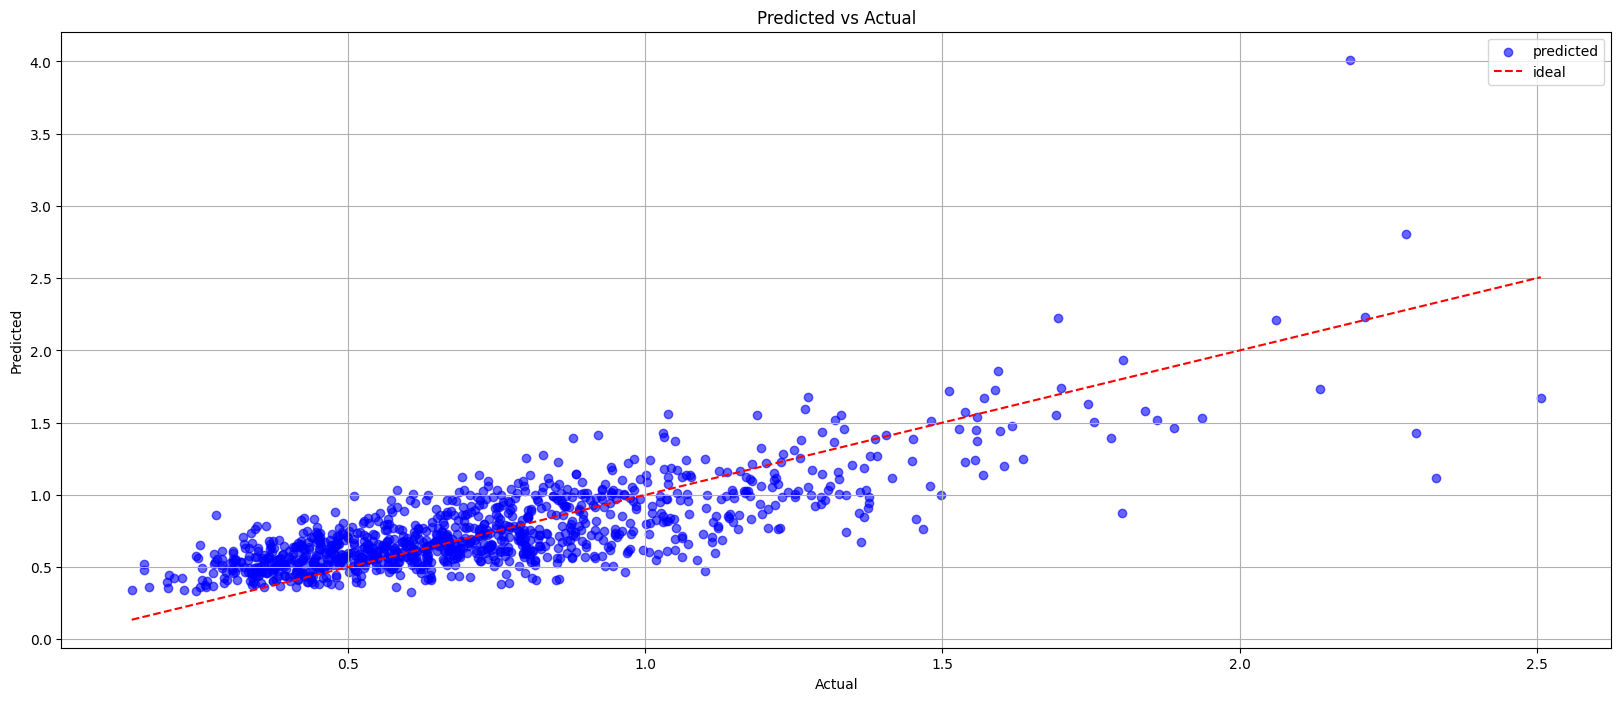
\includegraphics[width=0.9\textwidth]{img/PVA_R.png}
\end{center}

And the second neural network for option pricing compare to black scholes output :
\begin{center}
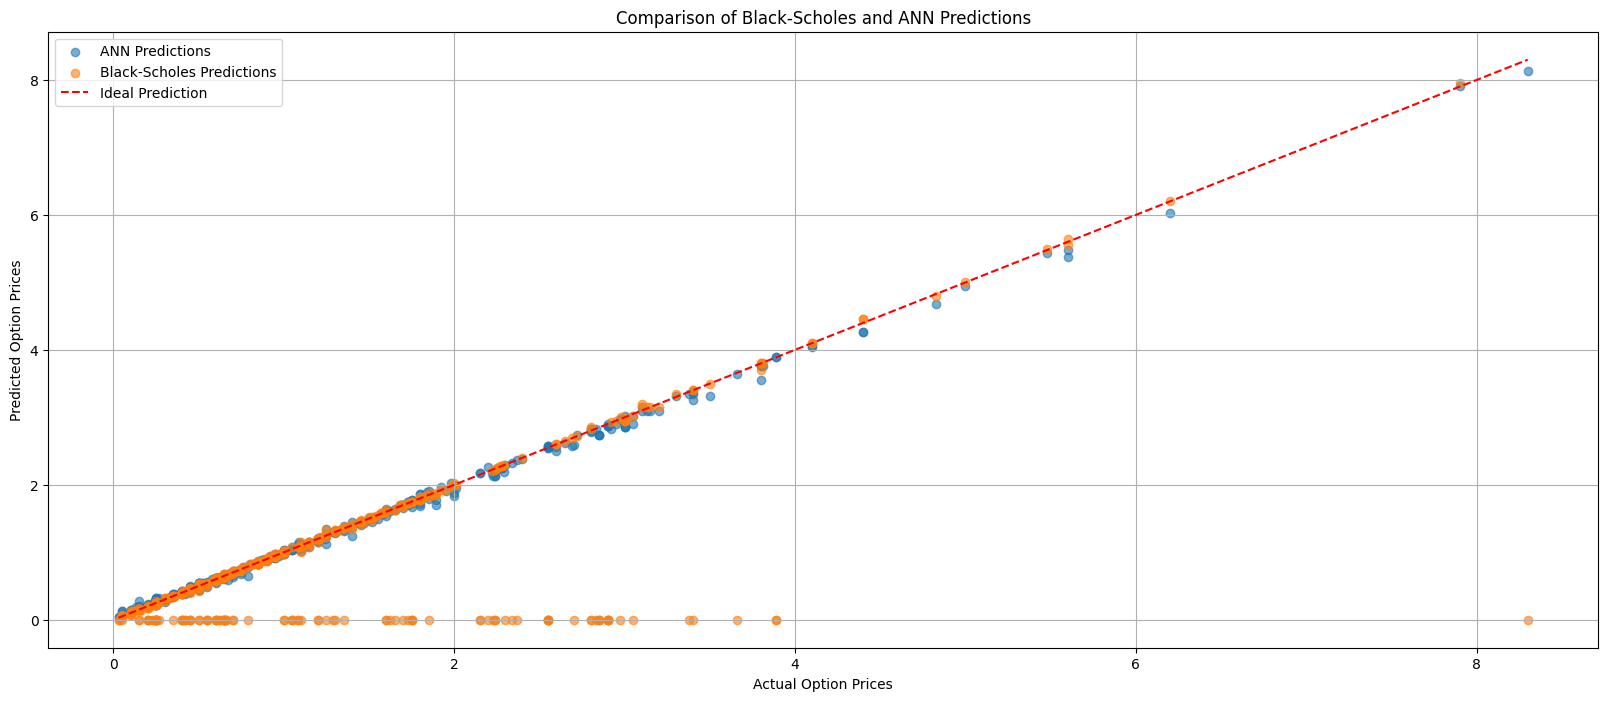
\includegraphics[width=0.9\textwidth]{img/BS_VS_ANN.png}
\end{center}


\section{Next Steps}

As stated in the results section, regression has been challenging for the models, with room for improvement despite decent regression evidence. This project will focus on improving volatility forecasting by ANN. The next step is to tune LSTM hyperparameters to improve its performance and gain the most from its memory advantage. Data work, like outlier suppression, will also be a fundamental aspect to build models and new methods on solid ground.



\begin{center}
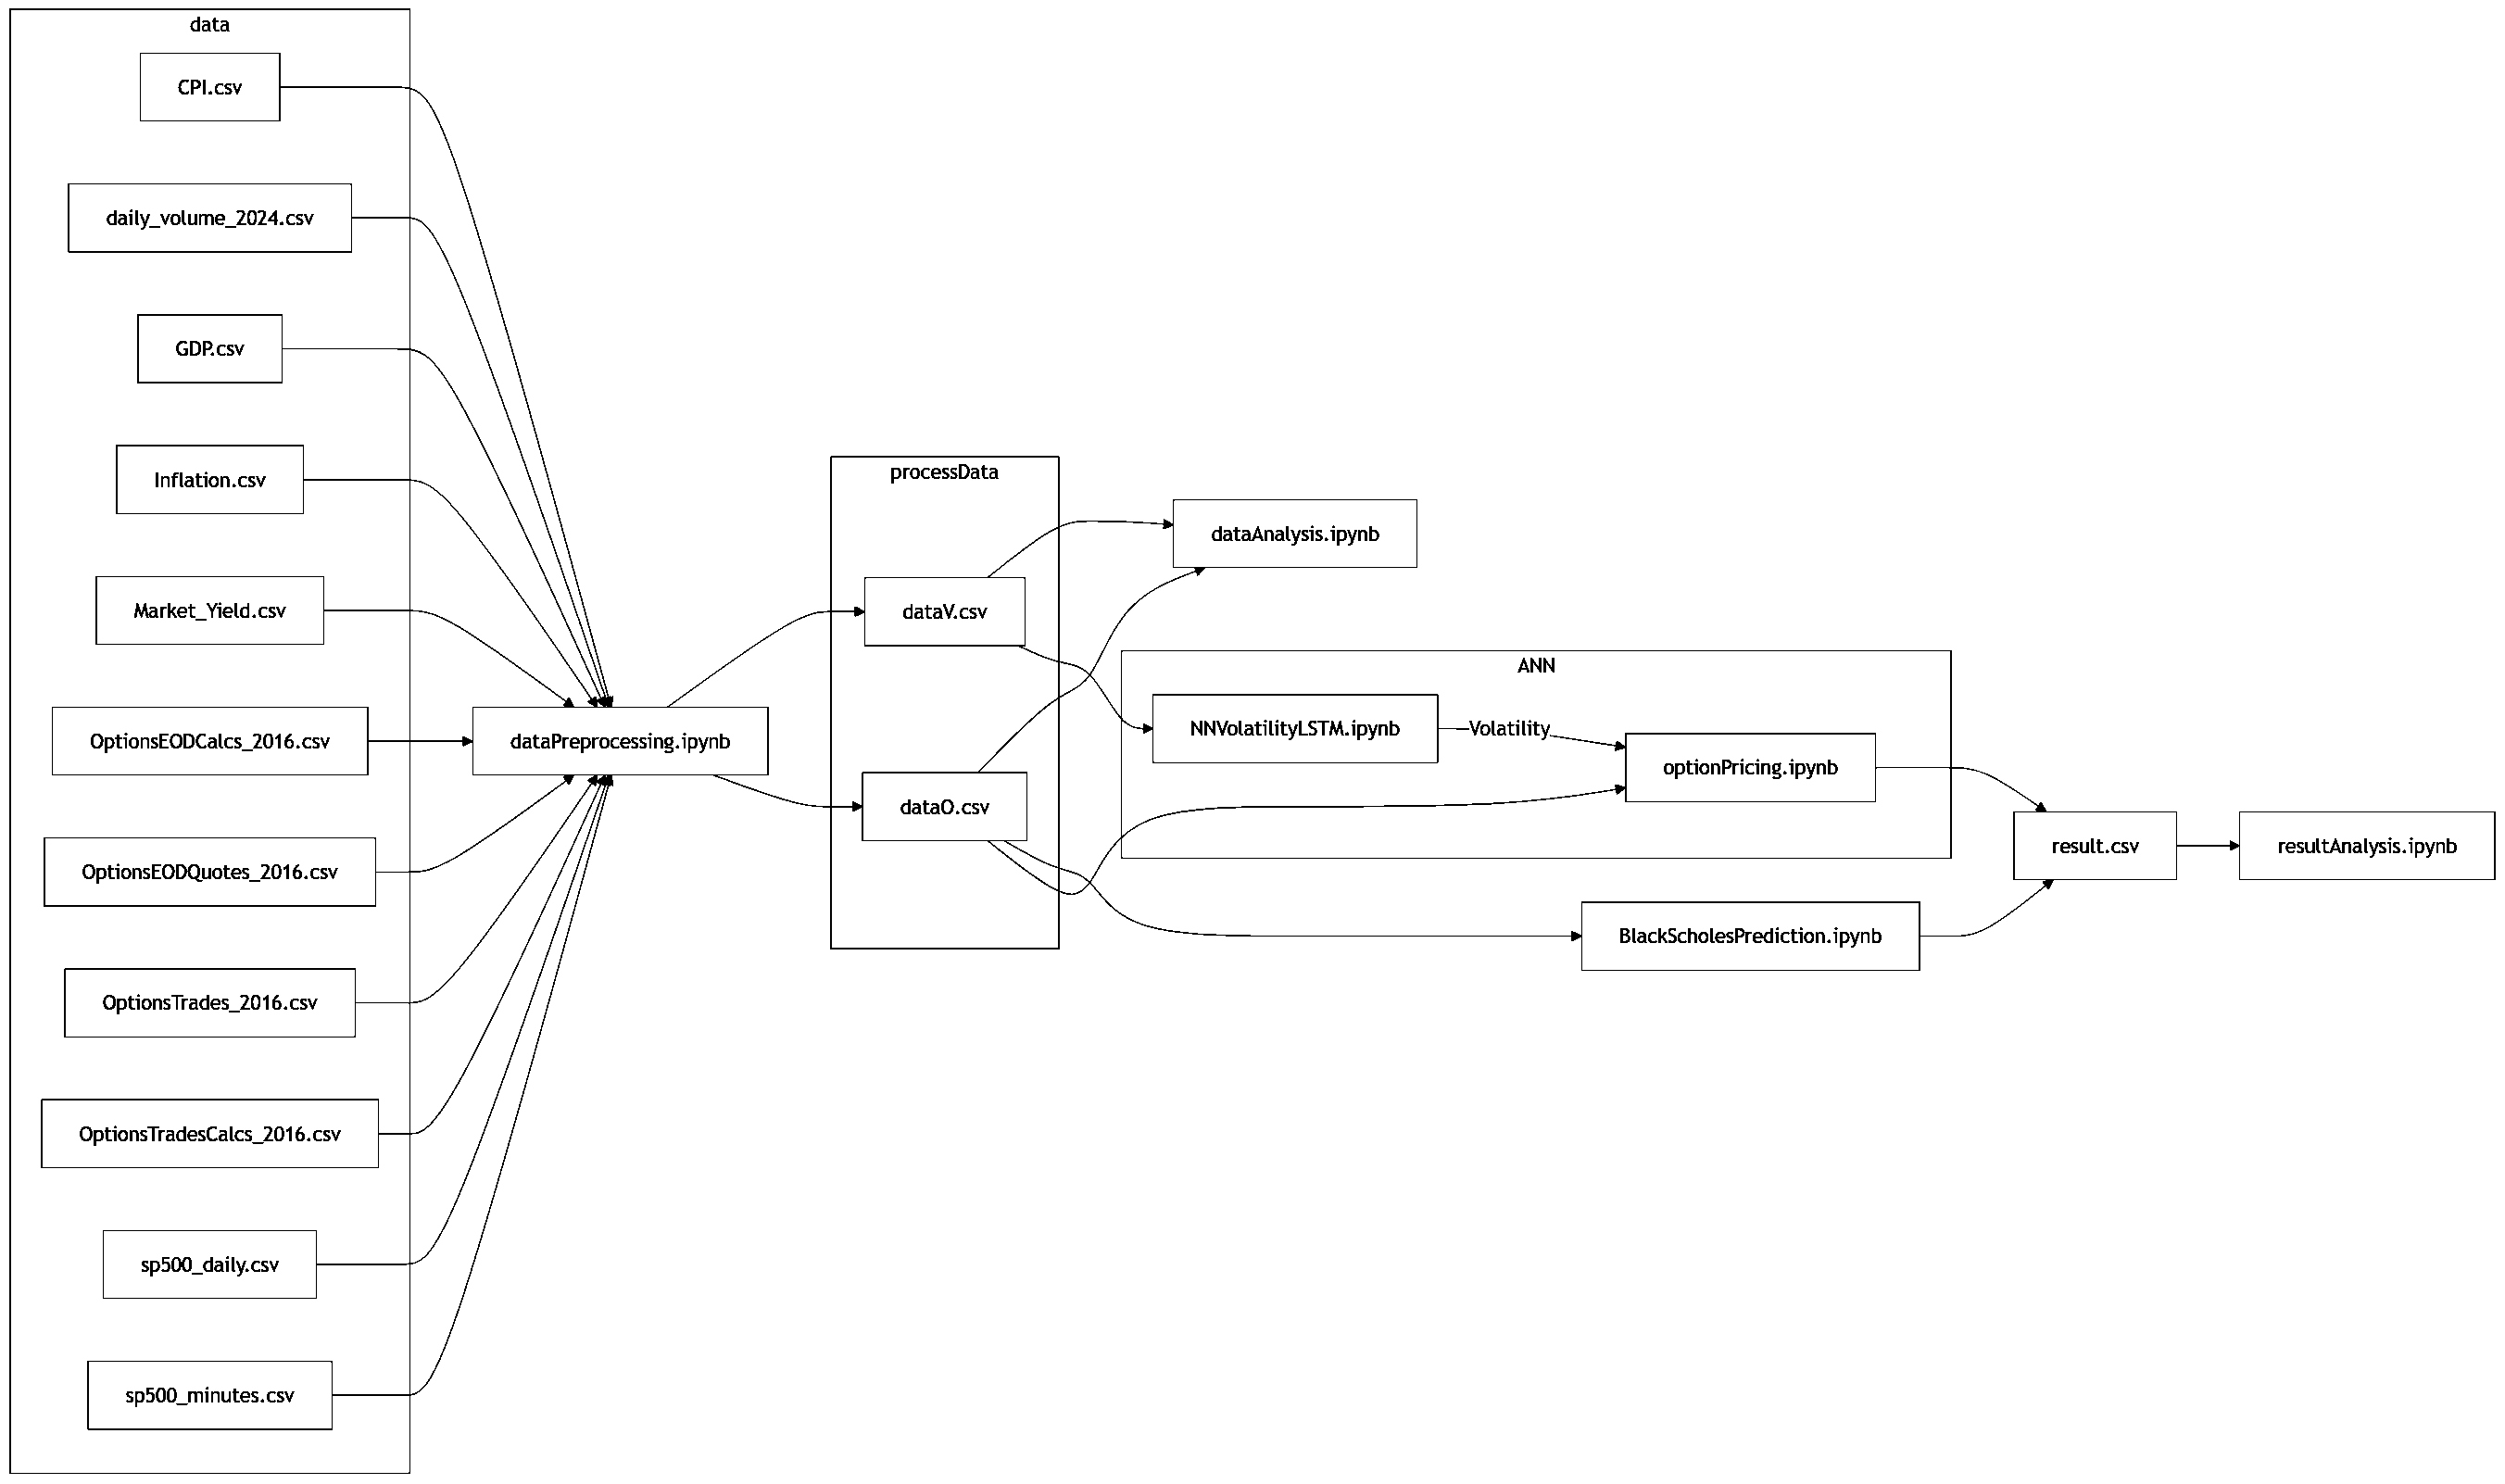
\includegraphics[width=1\textwidth]{img/structure_bw.png}
\end{center}





\end{document}
